\newcommand{\covtype}{\texttt{covtype}\xspace}
\newcommand{\sensit}{\texttt{sensit}\xspace}

% no longer in use
\newcommand{\resultcurves}[2]{
\begin{figure}[!h]
\centering
\subfigure[\covtype.]{\includegraphics[width=0.22\textwidth]{#1_covtype_pu_resvm.pdf}}\qquad
\subfigure[\sensit.]{\includegraphics[width=0.22\textwidth]{#1_sensit_2_semi_resvm.pdf}}\\
\caption{#2}
\label{fig:results-#1}
\end{figure}
}

\newcommand{\resultcurvesnew}[2]{
\begin{figure}[!h]
\centering
%\subfigure[Rank CDF for \covtype.]{\includegraphics[width=0.2\textwidth]{cdf_covtype_pu_resvm.pdf}}\qquad
%\subfigure[ROC curves for \covtype.]{\includegraphics[width=0.2\textwidth]{roc_covtype_pu_resvm.pdf}}\qquad
%\subfigure[PR curves for \covtype.]{\includegraphics[width=0.2\textwidth]{pr_covtype_pu_resvm.pdf}}
\subfigure[Rank CDF for \covtype.]{\includegraphics[width=0.2\textwidth]{#1_cdf.pdf}}\qquad
\subfigure[ROC curves for \covtype.]{\includegraphics[width=0.2\textwidth]{#1_roc.pdf}}\qquad
\subfigure[PR curves for \covtype.]{\includegraphics[width=0.2\textwidth]{#1_pr.pdf}}
\caption{#2}
\label{fig:results-#1}
\end{figure}
}

\section{Discussion and Recommendations}
Next, we discuss several issues related to using our approach in practice. 

\subsection{Determining $\hat{\pfrac}$ and its effect}

Our approach requires having an estimate $\hat{\pfrac}$ of $\pfrac$. There are many problems where $\pfrac$ is known from domain knowledge (e.g., calculated and published based on a data source you do not have access to), but explicit negatives are scarce or unavailable in the data under analysis. A real-world example where this is true is the task of predicting whether someone has diabetes from health insurance data (cfr. Chapter~\ref{ch:diabetesjmlr}). Some individuals are coded as having diabetes, but many diabetics are undiagnosed and hence it is wrong to assume that all unlabeled patients do not have diabetes. However, the incidence rate of diabetes is known and published in the medical literature. This type of situation characterizes many medical problems. If $\pfrac$ is not known from domain knowledge, then it could be estimated from data \citep{Elkan:2008:LCO:1401890.1401920, scottblanchard,scholkopf2001estimating}.

% are similar.

%- Direct marketing attempts to identify future customers from their profiles. Current customers are positive examples. Databases of unlabeled examples can be purchased at low cost (Lee \& Liu, ICML 2003). The fraction of potential customers in a population is often known. 

In either case, if $\hat{\pfrac}$ is not exact, the conditions of Lemma~\ref*{lemma-rank-fpr} are potentially violated where it is used within Theorem~\ref{main-theorem}. The effects of set size on FPR is characterized in Lemma~\ref*{lemma-size-fpr}, which will help us understand the effect of over or under estimating $\pfrac$.

%%%%%%%%%%%%%%%%%%%%%%%%%%%%%%%%%%%%%%%%%%%%%%%%%%
% 	LEMMA SIZE -> FPR
%%%%%%%%%%%%%%%%%%%%%%%%%%%%%%%%%%%%%%%%%%%%%%%%%%

\begin{lemma} \label{lemma-size-fpr}
Given two sets of positive labels $\pos_1$ and $\pos_2$ within an overall ranking $\overall$ and a rank $\ranksymb$, such that $\TPR(\pos_1,\ranksymb) = \TPR(\pos_2,\ranksymb)=t$ and $|\pos_1| > |\pos_2|$, then:
\begin{align*}
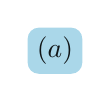
\begin{tikzpicture}[baseline=-0.5ex] \node [draw=none, fill=cyan!80!black, fill opacity=0.4, text opacity=0.9, rounded corners] (blah) {$(a)$}; \end{tikzpicture}
\quad \FPR(\pos_2, r) < \tprsymb &\rightarrow \FPR(\pos_1, r) < \FPR(\pos_2, r), \\
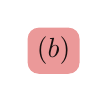
\begin{tikzpicture}[baseline=-0.5ex] \node [draw=none, fill=red!80!black, fill opacity=0.4, text opacity=0.9, rounded corners] (blah) {$(b)$}; \end{tikzpicture}
\quad \FPR(\pos_2, r) > \tprsymb &\rightarrow \FPR(\pos_1, r) > \FPR(\pos_2, r).
\end{align*}
(a) corresponds to a ranking and cutoff that is better than random (i.e. $\TPR(\pos,r) > \FPR(\pos,r)$) whereas (b) corresponds to a ranking and cutoff that is worse than random.

\begin{figure}[!h]
  \centering
  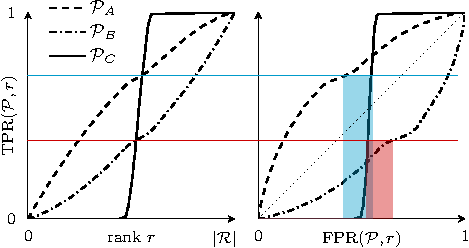
\includegraphics[width=0.6\textwidth]{lemma_size_fpr.pdf}
  \caption[]{Illustration of Lemma~\ref*{lemma-size-fpr}, with $\pos_A \subset \overall$, $\pos_B \subset \overall$, $\pos_C \subset \overall$, 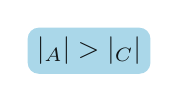
\begin{tikzpicture}[baseline=-0.5ex] \node [draw=none, fill=cyan!80!black, fill opacity=0.4, text opacity=0.9, rounded corners] (blah) {$|\pos_A| > |\pos_C|$}; \end{tikzpicture} and 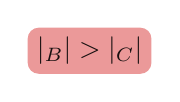
\begin{tikzpicture}[baseline=-0.5ex] \node [draw=none, fill=red!80!black, fill opacity=0.4, text opacity=0.9, rounded corners] (blah) {$|\pos_B| > |\pos_C|$}; \end{tikzpicture}. If two sets of positives $\pos_1$ and $\pos_2$ achieve a given TPR at the same rank $r$, e.g. $\TPR(\pos_1,r)=\TPR(\pos_2,r)$ and $|\pos_1| > |\pos_2|$ then $\FPR(\pos_1,r) < \FPR(\pos_2,r)$ if $\FPR(\pos_2,r) < \TPR(\pos_2,r)$ and otherwise $\FPR(\pos_1,r) > \FPR(\pos_2,r)$.} 
  \label{fig:lemma-size-fpr}
\end{figure}

\textbf{Proof}: take the derivative of FPR to $|\pos|$ while fixing $\ranksymb$, based on Equation~\eqref{tpr-fpr}:
\begin{align}
\frac{d\FPR(\pos, \ranksymb)}{d|\pos|} &= \frac{\ranksymb-\tprsymb\cdot|\overall|}{(|\overall|-|\pos|)^2}, \nonumber \\
&= \frac{\ranksymb-\tprsymb\cdot|\pos| - \tprsymb \cdot|\overall-\pos|}{(|\overall|-|\pos|)^2}. \label{FPR_ifv_gamma}
\end{align}
$r-\tprsymb\cdot|\pos|$ is the number of negatives in the top ranking (false positives) and $\tprsymb\cdot|\overall - \pos|$ is the number of false positives at $\FPR=\tprsymb$. The derivative is negative if the $\FPR$ is below $\tprsymb$ and vice versa, therefore if the ranking is better than random ($\TPR = \tprsymb > \FPR$), increasing $|\pos|$ leads to a lower $\FPR$ at rank $\ranksymb$ and vice versa. \hfill $\blacksquare$
\end{lemma}

Lemma~\ref*{lemma-size-fpr} has a large practical impact. If the ranking of $\knownpos$ is better than random, then over and under estimating $\hat{\pfrac}$ is useful to obtain a (loose) upper/lower bound on performance curves, respectively. In other words, given bounds or a CI on $\pfrac$, that is $\hat{\pfrac}_{lo} \leq \pfrac \leq \hat{\pfrac}_{up}$, we can use $\hat{\pfrac}_{lo}$ and $\hat{\pfrac}_{up}$ to estimate a lower and upper bound on the true ROC or PR curve. Bounds computed based on a CI for $\pfrac$ constitute a CI for the performance metric (at the same confidence level), assuming the rank CDF of $\latentpos$ is contained by the confidence band on the rank CDF. Tighter bounds on $\pfrac$ translate directly to tighter bounds on performance estimates. Finally, treating the full unlabeled set as negative results underestimates performance, since $\hat{\pfrac}=0 < \pfrac$. The effect of varying $\hat{\pfrac}$ is shown in Figure~\ref{fig:roc-ifv-beta}.

\begin{figure}[!h]
	\centering
	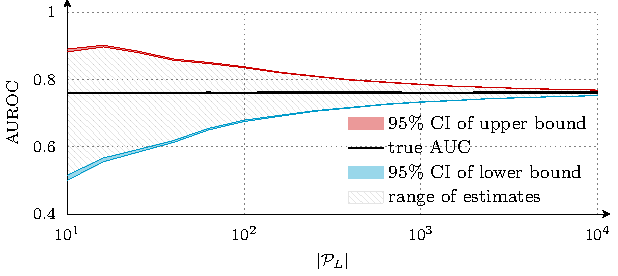
\includegraphics[width=0.8\textwidth]{convergence.pdf}
	\vfill	
	\caption{The effect of $|\knownpos|$ on estimated AUC. Based on $|\unlabeled| = 100,000$, $\knownneg=\emptyset$ and $\hat{\pfrac}=\pfrac=0.2$. Bounds on rank CDF were obtained via bootstrap. The depicted confidence intervals are based on 200 repeated experiments.}
	\label{fig:convergence}
\end{figure}
\begin{figure}[!h]
	\centering
	\centering
	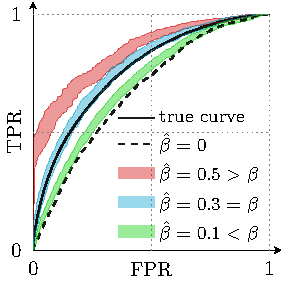
\includegraphics[width=0.4\textwidth]{roc_ifv_beta.pdf}
	\vfill
	\caption{The effect of $\hat{\pfrac}$ on estimated ROC curves, based on 2,000 known positives, 100,000 unlabeled instances and $\pfrac=0.3$.}
	\label{fig:roc-ifv-beta}
\end{figure}

%Given the relationship between ROC and PR curves as explained in Section~\ref{roc-pr}, the pattern in Figure~\ref{fig:roc-ifv-beta} applies to PR curves too: overestimating $\hat{\pfrac}$ results in overly optimistic bounds (can yield a loose upper bound) while underestimating $\hat{\pfrac}$ results in pessimistic bounds (can yield a loose lower bound).

\subsection{Model selection}
Often evaluation metrics are used to select the best model from a set of candidates. If model A's ROC (PR) curve dominates model B's ROC (PR) curve, then for all $\pfrac$ model A is better than model B (leaving aside significance testing). However, in most cases one model does not dominate another model and there exists a point where the two curves cross. Surprisingly, the ordering in terms of both AUROC and AUPR are dependent on $\hat{\pfrac}$ when this happens. This means that the ordering of models according to these metrics can switch when $\hat{\pfrac}$ changes. Figure~\ref{rocauc-switch} depicts an example that illustrates this. This demonstrates that $\hat{\pfrac}$ can play a crucial role in model selection. In the likely event that the curves cross, it is important to look at the range of possible values for $\hat{\pfrac}$ that represent different operating conditions when selecting among different models.

%there is strict dominance ordering of the models, that is, for a given FPR, model A's TPR is always greater than or equal to model B's TPR, then 


A more formal explanation of why this occurs can be made based on partial derivatives of each entry of the partial contingency table and TPR, FPR and precision based on unlabeled instances to $\hat{\pfrac}$:\footnote{We made some simplifications, the details are described in Appendix~\ref*{partial}.}
\begin{align}
\frac{\partial \TPR_U^r}{\partial \hat{\pfrac}} &= 0,\\
\frac{\partial \FPR_U^r}{\partial \hat{\pfrac}} &= \frac{|\topfun(\unlabeled, r)| - \mathcal{T}(r) \cdot |\unlabeled|}{(1-\hat{\pfrac})^2}, \label{eq:partials} \\
\frac{\partial \PREC_U^r}{\partial \hat{\pfrac}} &= \frac{\mathcal{T}(r)\cdot|\unlabeled|}{|\topfun(\unlabeled,r)|} \geq 0.
\end{align}
The partial derivative of TPR is exactly 0 because our approach is based on rank CDFs (that is TPR at each rank). Interestingly, the partial derivatives of FPR and precision to $\hat{\pfrac}$ are dependent on the value of the rank CDF $\mathcal{T}(r)$ that is being used to infer surrogate positives. Since $\TPR$ is not a function of $\hat{\pfrac}$ and the partial derivatives of $\FPR$/precision to $\hat{\pfrac}$ are functions of $\mathcal{T}(r)$, distinct segments of an ROC/PR curve are moved differently when $\hat{\pfrac}$ changes, inducing a non-uniform scaling of AUC across the TPR range. Such scaling potentially changes the ordering of models based on AUC. 
% property. 

%Model selection aims to identify the best model from a set of candidates and involves a series of pair-wise comparisons of classifiers $A$ and $B$ to decide which is best, based on empirical measurements of some metric such as AUROC. Each model is characterized by the rank CDF of known positives based on that model's predictions, that is $\mathcal{T}_A(r)$ and $\mathcal{T}_B(r)$. The rank CDF is used to infer surrogate positives $\surrpos$ from the unlabeled set $\unlabeled$ in order to estimate the performance metric of interest. 

%Since $\TPR$ is not a function of $\hat{\pfrac}$ and the partial derivative of $\FPR$ to $\hat{\pfrac}$ is a function of $\mathcal{T}(r)$, distinct segments of an ROC curve are moved differently when $\hat{\pfrac}$ changes, inducing a non-uniform scaling of AUC across the TPR range. A direct result of this observation is that the best model in terms of AUROC is contingent on $\hat{\pfrac}$, i.e. it is possible for a model to become better than another in terms of AUROC when $\hat{\pfrac}$ changes, given that the rank distributions $\mathcal{T}_A(r)$ and $\mathcal{T}_B(r)$ of both models cross. The sensitivity of AUROC to $\hat{\pfrac}$ depends on the shape of the curve.  The same reasoning applies to PR curves, since the partial derivative of precision to $\hat{\pfrac}$ is also a function of $\mathcal{T}(r)$. This proves that good estimates of $\hat{\pfrac}$ are necessary for correct model selection (and hence, using $\hat{\pfrac}=0$ to perform model selection is suboptimal). Figure~\ref{rocauc-switch} depicts an example illustrating this property. 
\begin{figure}[!h]
\centering
  \begin{minipage}[c]{0.45\textwidth}
  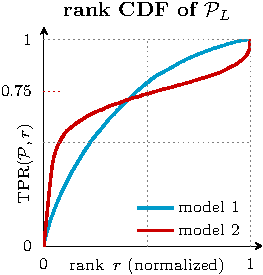
\includegraphics[width=\textwidth]{switch_cdf.pdf}
  \end{minipage}\hfill
  \begin{minipage}[c]{0.45\textwidth}
  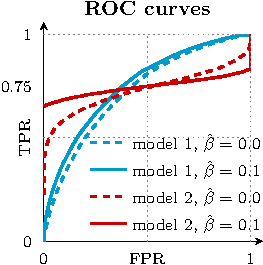
\includegraphics[width=\textwidth]{switch_roc.pdf}
  \end{minipage}
\caption[]{The effect of $\hat{\pfrac}$ on ROC curves. Setup: $|\unlabeled|=45,000$, $|\knownpos|=5,000$. \\%Model 2 wins for $\hat{\pfrac}=0$, but model 1 wins for $\hat{\pfrac}=0.1$. %The curve for model 2 is independent of $\hat{\pfrac}$. 

Corresponding AUROC (best in bold): 
{\centering
\begin{tabular}{ccc}
\toprule
estimated $\hat{\pfrac}$ 	& model 1 	& model 2 \\
\midrule
0.0		& $72.5\%$		& $\mathbf{73.2\%}$ \\
0.1		& $\mathbf{75.5\%}$	& $74.7\%$ \\
\bottomrule
\end{tabular}}
}\label{rocauc-switch}
\end{figure}


\subsection{Empirical quality of the estimates} \label{empirical}
We illustrate the quality of our estimated bounds on ROC and PR curves using a model trained in a PU learning setting \citep{Claesen2015resvm} on the \covtype data set \citep{Blackard00covtype}. The model was evaluated on a fully labeled test set of $20,000$ positive and $20,000$ negative examples. To estimate performance, we randomly selected $5\%$ of positive examples to serve as our labeled set and treated all other examples as unlabeled, which yields $|\knownpos|=1,000$, $|\unlabeled| = 39,000$ and $\pfrac\approx49\%$. We present ROC and PR curves with bounds for $\hat{\pfrac}=\pfrac$, $\hat{\pfrac}=0$, and a confidence interval $\hat{\pfrac}_{lo} = 0.8\pfrac \leq \hat{\pfrac} \leq \hat{\pfrac}_{up} = 1.2\pfrac$. Finally, as we have the ground truth, we present true curves as a reference.\footnote{Python code to reproduce all results (and modify the configuration) is available at \url{https://github.com/claesenm/semisup-metrics}.}

Figure~\ref{fig:results-covtype} presents  the rank CDF and estimated bounds on ROC and PR curves. Figure~\ref{fig:results-covtype-cdf} shows the true rank CDF of $\latentpos$ along with an estimated $95\%$ CI on the rank CDF using the $\knownpos$ via a standard bootstrap approach with $2,000$ resamples. In this case, the CI contains the true rank CDF of latent positives.\footnote{The rank CDF of $\latentpos$ is unknown in practice, but assumed to be comparable to the rank CDF of $\knownpos$.} Figures~\ref{fig:results-covtype-roc} and~\ref{fig:results-covtype-pr} show that the bounds closely approximate the true performance curves. The estimated bounds are wider in PR space than in ROC space, particularly at low recall. Note that estimated PR curves are sensitive to the estimation error in $\hat{\pfrac}$, as precision is directly affected by class balance, limiting their usefulness if only a rough estimate of $\pfrac$ is available.

%Figure~\ref{fig:results-covtype} presents the rank CDF and estimated bounds on ROC and PR curves. Figure~\ref{fig:results-covtype-cdf} shows the true rank CDF along with an estimated $95\%$ CI on the rank CDF using the $\knownpos$ via a standard bootstrap approach with $2,000$ resamples. In this case, the CI contains the true rank CDF of latent positives (which is unknown in practice). Hence, the true ROC and PR curves assuming all labels are know are guaranteed to be between the bounds estimated using the partial labeled data, assuming that $\hat{\pfrac}_{lo} \leq \pfrac \leq \hat{\pfrac}_{up}$. This can be confirmed in Figures~\ref{fig:results-covtype-roc} and~\ref{fig:results-covtype-pr}.

%The bounds closely approximate the true performance curves, depending on the quality of $\hat{\pfrac}$ and the width of the CI on rank CDF. The estimated bounds are wider in PR space than in ROC space, particularly at low recall (Figure~\ref{fig:results-covtype-pr} and~\ref{fig:results-covtype-roc}, respectively). Additionally, it must be noted that estimated PR curves are very sensitive to the estimation error in $\hat{\pfrac}$, because precision is directly affected by class balance. As such, we recommend using ROC curves over PR curves when only a rough estimate of $\pfrac$ is available.



\begin{figure}%
\centering
\subfloat[Rank CDF.\label{fig:results-covtype-cdf}]{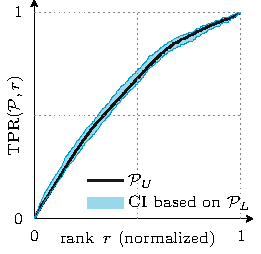
\includegraphics[width=0.31\textwidth]{covtype_cdf.pdf}}\hfill
\subfloat[ROC curves.\label{fig:results-covtype-roc}]{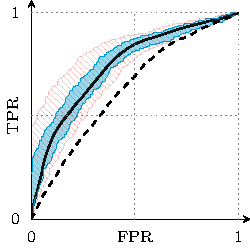
\includegraphics[width=0.31\textwidth]{covtype_roc.pdf}}\hfill
\subfloat[PR curves.\label{fig:results-covtype-pr}]{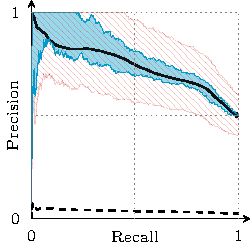
\includegraphics[width=0.31\textwidth]{covtype_pr.pdf}}\\
\caption[]{Results for \covtype showing rank CDF, ROC and PR curves, with $\pfrac\approx 49\%$.
Performance curve legend:  \newline
\begin{tikzpicture}[baseline=-0.5ex] \draw [color=black, thick] (0, 0) -- (0.5, 0); \end{tikzpicture} true curve, 
\begin{tikzpicture}[baseline=-0.5ex] \draw [color=black, thick, dashed] (0, 0) -- (0.5, 0); \end{tikzpicture} $\hat{\pfrac}=0$, 

\begin{tikzpicture}[baseline=-0.5ex] \draw [color=cyan!80!black, opacity=0.8] (0, -0.2) rectangle (0.7, 0.3); 
\fill [color=cyan!80!black, opacity=0.4] (0, -0.2) rectangle (0.7, 0.3); \end{tikzpicture} $\hat{\pfrac}=\pfrac$ and 
\begin{tikzpicture}[baseline=-0.5ex] \draw [color=red!80!black, opacity=0.2, pattern=north west lines, pattern color=red!80!black] (0, -0.2) rectangle (0.7, 0.3); \end{tikzpicture} $0.8\pfrac \leq \hat{\pfrac} \leq 1.2\pfrac$.}
\label{fig:results-covtype}
\end{figure}

\ifx
\begin{figure}[h]
\centering
\subfigure[Rank CDF.\label{fig:results-covtype-cdf}]{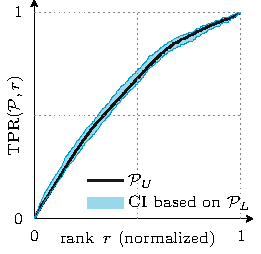
\includegraphics[width=0.25\textwidth]{covtype_cdf.pdf}}\qquad
\subfigure[ROC curves.\label{fig:results-covtype-roc}]{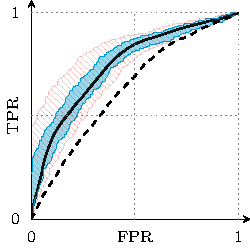
\includegraphics[width=0.25\textwidth]{covtype_roc.pdf}}\qquad
\subfigure[PR curves.\label{fig:results-covtype-pr}]{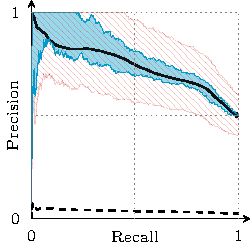
\includegraphics[width=0.25\textwidth]{covtype_pr.pdf}}
\addtolength{\abovecaptionskip}{-3mm}
%\subfigure[Rank CDF for \sensit.]{\includegraphics[width=0.29\textwidth]{cdf_sensit_2_semi_resvm.pdf}}\qquad
%\subfigure[ROC curves for \sensit.]{\includegraphics[width=0.29\textwidth]{roc_sensit_2_semi_resvm.pdf}}\qquad
%\subfigure[PR curves for \sensit.]{\includegraphics[width=0.29\textwidth]{pr_sensit_2_semi_resvm.pdf}}
%\caption{Results for \covtype and \sensit showing rank CDF, ROC and PR curves (left to right).}
\caption[]{Results for \covtype showing rank CDF, ROC and PR curves, with $\pfrac\approx 49\%$. \newline
Performance curve legend: 
\begin{tikzpicture}[baseline=-0.5ex] \draw [color=black, thick] (0, 0) -- (0.5, 0); \end{tikzpicture} true curve, 
\begin{tikzpicture}[baseline=-0.5ex] \draw [color=black, thick, dashed] (0, 0) -- (0.5, 0); \end{tikzpicture} $\hat{\pfrac}=0$, 

\begin{tikzpicture}[baseline=-0.5ex] \draw [color=cyan!80!black, opacity=0.8] (0, -0.2) rectangle (0.7, 0.3); 
\fill [color=cyan!80!black, opacity=0.4] (0, -0.2) rectangle (0.7, 0.3); \end{tikzpicture} $\hat{\pfrac}=\pfrac$ and 
\begin{tikzpicture}[baseline=-0.5ex] \draw [color=red!80!black, opacity=0.2, pattern=north west lines, pattern color=red!80!black] (0, -0.2) rectangle (0.7, 0.3); \end{tikzpicture} $0.8\pfrac \leq \hat{\pfrac} \leq 1.2\pfrac$.}
\label{fig:results-covtype}
\addtolength{\abovecaptionskip}{3mm}
\end{figure}
\fi


%positive labels (chosen at random), ignored all negative labels along with $95\%$ of positive labels (chosen at random), which yields $|\knownpos|=1,000$, $|\unlabeled| = 39,000$ and $\pfrac\approx49\%$. We have computed bounds on the ROC and PR curves based on treating $\unlabeled$ as negative (i.e., $\hat{\pfrac}=0$), the right amount of latent positives (i.e., $\hat{\pfrac}=\pfrac$) and a confidence interval ($\hat{\pfrac}_{lo} = 0.8\pfrac \leq \hat{\pfrac} \leq \hat{\pfrac}_{up} = 1.2\pfrac$). Having all test labels enabled us to compute true performance curves as a reference. \footnote{Python code to reproduce all results (and modify the configuration) is available as supplementary material.}

 %(consisting of $20,000$ positives and negatives). Having all test labels enabled us to compute true performance curves as a reference. 



%To illustrate our approach, we estimated bounds on ROC and PR curves and compared these to the ground truth. We used rankings and corresponding true labels of simulations done by BLINDED, in which classifiers were tuned and trained in a PU learning context on the \covtype data set \citep{Blackard00covtype} and tested on an independent, fully labeled test set (consisting of $20,000$ positives and negatives). Having all test labels enabled us to compute true performance curves as a reference. 

%To produce our estimations, we ignored all negative labels along with $95\%$ of positive labels (chosen at random), which yields $|\knownpos|=1,000$, $|\unlabeled| = 39,000$ and $\pfrac\approx49\%$. We have computed bounds on the ROC and PR curves based on treating $\unlabeled$ as negative (i.e., $\hat{\pfrac}=0$), the right amount of latent positives (i.e., $\hat{\pfrac}=\pfrac$) and a confidence interval ($\hat{\pfrac}_{lo} = 0.8\pfrac \leq \hat{\pfrac} \leq \hat{\pfrac}_{up} = 1.2\pfrac$). Python code to reproduce all results (and modify the configuration) is available as supplementary material.

%Figure~\ref{fig:results-covtype} shows the rank CDF and estimated bounds on ROC and PR curves. We estimated a $95\%$ CI on the rank CDF of $\knownpos$ via a standard bootstrap approach, using $2,000$ resamples. As the confidence band on rank CDF contains the true rank CDF of latent positives (which is unknown in practice), the true ROC and PR curves (based on $\bothpos$) are guaranteed to be between the respective bounds (based on $\bothposapprox$), given $\hat{\pfrac}=\pfrac$ or $\hat{\pfrac}_{lo} \leq \pfrac \leq \hat{\pfrac}_{up}$, as is confirmed by the results in Figure~\ref{fig:results-covtype}.

%The bounds closely approximate the true performance curves, depending on the quality of $\hat{\pfrac}$. The estimated bounds are wider in PR space than in ROC space, particularly at low recall (Figure~\ref{fig:results-covtype-pr} and~\ref{fig:results-covtype-roc}, respectively). Additionally, it must be noted that estimated PR curves are very sensitive to the estimation error in $\hat{\pfrac}$, because precision is directly affected by class balance. As such, we recommend using ROC curves over PR curves when only a rough estimate of $\pfrac$ is available.


\subsection{Relative importance of known negatives compared to known positives}
As our approach can incorporate known negatives, a natural question is how their presence influences the estimates. In practice, a test set is of fixed size, so known negatives essentially reduce the size of the unlabeled subset, which in turn reduces the number of degrees of freedom in assigning surrogate positives. Using the same setup as in Subsection~\ref{empirical}, we varied the proportion of known positives and negatives and found known negatives provide some benefit, though this is small in practice. However, our approach can also be reversed given a large amount of negatives, that is flip known class labels, use $\bar{\pfrac}=1-\pfrac$ and adjust the resulting contingency tables accordingly, which can improve performance bounds. The benefits of known negatives are further discussed in Appendix~\ref*{knownneg}.




%benefit does their presence

%n

%nown negatives can b incorporated in our approach as described in Section~\ref{contingency}. Given a fixed ranking $\overall$, having known negatives essentially reduces the size of the unlabeled subset $\unlabeled$, which in turn reduces the number of degrees of freedom in assigning surrogate positives. As such, known negatives provide some benefit, though this is small in practice (see Appendix~\ref*{knownneg} for an example).

%However, when the number of known negatives is large enough our approach can be reversed, that is flip known class labels, use $\pfrac$ to $\bar{\pfrac}=1-\pfrac$ and adjust the resulting contingency tables accordingly. Hence, bounds can be computed based primarily on known positives $\knownpos$ \emph{or} known negatives $\knownneg$. The width of the bounds depends on the combination of $|\knownpos|$ (or $|\knownneg|$) and $\pfrac$ (or $\bar{\pfrac}$) in a nontrivial way: depending on $\pfrac$, it is possible to obtain wider bounds based on known negatives, even if $|\knownneg| > |\knownpos|$ (or vice versa). In practice, we can estimate metrics based on $\knownpos$ and $\knownneg$ separately and then use whichever yields the tightest bounds. More information is included in Appendix~\ref*{knownneg}.

\section{Conclusion}
We presented an approach to construct contingency tables corresponding to a lower and upper bound on FPR using only partially labeled, which enables computing many commonly used performance metrics in a semi-supervised setting. Our approach relies on knowing the fraction of latent positives in the unlabeled data, and we discussed its effect on determing the bounds and model selection. We have seen that our approach can yield good estimates in practice.  

%at a given rank based on a confidence interval on the rank CDF of (known) positives. Via these estimated contingency tables many commonly used performance metrics become available in a semi-supervised setting. We have shown that the bounds enable proper model evaluation, though model selection based on AUROC requires good estimates of the fraction of latent positives in the unlabeled set ($\pfrac$). Poor estimates of $\pfrac$ may invalidate the bounds and hamper model selection.

%Our approach was used to compute bounds on ROC and PR curves in a realistic experiment, the quality of which is limited only by the quality of estimated confidence intervals on the CDF of ranks of positives and the estimated fraction of latent positives $\hat{\pfrac}$. Due to the sensitivity of the bounds in PR space to $\hat{\pfrac}$, we recommend using ROC curves for model evaluation in a partial labeling context. 
